\section{Echtzeitvisualisierung und OpenGL}
\subsection{Geschichte}
OpenGL entstand ursprünglich aus dem von Silicon Graphics (SGI) entwickelten IRIS GL. Im sogenannten Fahrenheit-Projekt versuchten Microsoft und SGI ihre 3D-Standards zu vereinheitlichen, das Projekt wurde jedoch wegen finanzieller Schwierigkeiten auf Seiten von SGI abgebrochen.

Der OpenGL-Standard wird vom OpenGL ARB (Architecture Review Board) festgelegt. Das ARB existiert seit 1992 und besteht aus einer Reihe von Firmen. Stimmberechtigte Mitglieder sind die Firmen 3DLabs, Apple, AMD/ATI, Dell, IBM, Intel, Nvidia, SGI und Sun (Stand Nov. 2004). Weiter mitwirkende Firmen sind Evans and Sutherland, Imagination Technologies, Matrox, Quantum3D, S3 Graphics, Spinor GmbH, Tungsten Graphics, und Xi Graphics. Microsoft, eines der Gründungsmitglieder, hat das ARB im März 2003 verlassen.

Neue Funktionen in OpenGL werden meist zuerst als herstellerspezifische Erweiterungen eingeführt und gehen dann den Weg über herstellerübergreifende Erweiterungen und ARB-Erweiterungen zu Kernfunktionalität. Dies erlaubt es, neueste Möglichkeiten der Grafikhardware zu nutzen und dennoch OpenGL abstrakt genug zu halten.

Quelle: https://de.wikipedia.org/wiki/OpenGL
\subsection{GL-Pipeline}
Eine Computergrafik-Pipeline besteht im Wesentlichen aus den folgenden Schritten:
\begin{figure}[H]
    \centering
    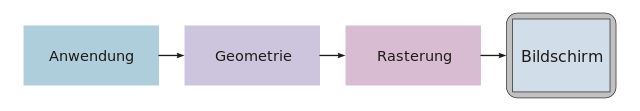
\includegraphics[width=1.0\textwidth]{images/cgpipeline_grob.png}
    \caption{Computergrafik-Pipeline}
    \label{fig:cdpipeline-overview}
\end{figure}


Eine solche Pipeline wird auch von OpenGL implementiert. Es besteht jedoch die Besonderheit, dass die Geometrie und die  Rasterung in Hardware realisiert ist und man durch kleine Programme, sogenannte Shader, auf diese Hardware zugreifen und Manipulationen vornehmen kann beziehungsweise seit OpenGL 2.0 sogar muss.

\subsubsection{Opengl Shaderpipeline}
\begin{figure}[H]
	\centering
	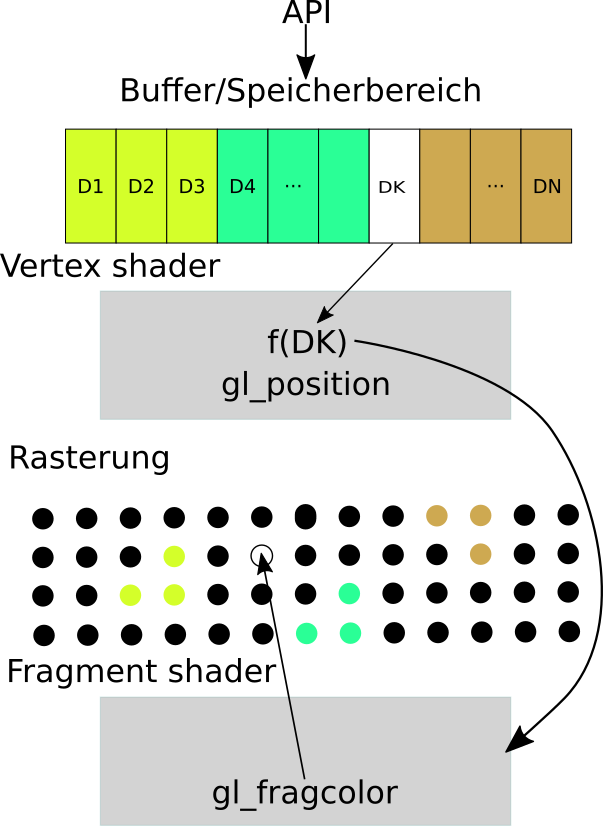
\includegraphics[width=1.0\textwidth]{images/Zeichnung_Shaderpipeline.png}
	\caption{Zentralprojektion}
	\label{fig:projection-sight-vol}
\end{figure}


\subsubsection{Geometrie}
Die Geometrieverarbeitung   besteht aus der Hintereinanderausführung der folgenden affinen/homogenen Abbildungen und Algorithmen:
\begin{figure}[H]
    \centering
    \includegraphics[width=1.0\textwidth]{images/cgpipeline.png}
    \caption{Geometrie-Pipeline}
    \label{fig:cgpipeline-geometry}
\end{figure}

\subsubsection*{Modell und Kameratransformationen}
Die Transformationen von Objektkoordinaten in das Kamerakoordinatensystem werden durch affine Transformationen beschrieben, welche durch Multiplikation durch homogene $4 \times 4$-Matrizen realisiert werden. 

\subsubsection*{Projektion}
Die Projektion wird durch Matrizen ähnlich der Projektionsmatrix 
$K_{persp_{xy}}$ und $K_{orth_{xy}}$ aus Abschnitt 
\ref{subsub:math:affine-space:homog-coords-projection} realisiert. 
Es werden jedoch noch  Translationen, Rotationen und Stauchungen 
dazwischen geschaltet, die ebenfalls als $4 \times 4$-Matrizen realisiert werden 
können und mit denen diese Matrix multipliziert werden. 
Man erreicht damit, dass der Kegelstumpf zwischen der vorderen 
(\textit{nearplane}) und der hinteren (\textit{farplane}) Projektionsebene in 
den $[-1,1] \times [-1,1] \times [-1,1] $ Würfel abgebildet wird, welcher auch 
Sichtvolumen genannt wird. 

\begin{figure}[H]
    \centering
    \includegraphics[width=1.0\textwidth]{images/gl_projectionmatrix01.png}
    \caption{Projektion und Sichtvolumen}
    \label{fig:projection-sight-vol}
\end{figure}

\begin{figure}[H]
    \centering
    \includegraphics[width=0.5\textwidth]{images/gl_projectionmatrix03.png}
    \caption{Zentralprojektion}
    \label{fig:projection-sight-vol}
\end{figure}
Die Multiplikation all dieser Matrizen wird auch die MODEL-VIEW-PROJECTION-MATRIX genannt. 

In obigen Fall ist die Projektionsmatrix gegeben  geben durch 
\begin{align*}
P := \begin{pmatrix}  
\frac{2n}{r-l}  &  0 &  \frac{r+l}{r-l}  & 0  \\
0   &  \frac{2n}{t-b} & \frac{t+b}{t-b} & 0  \\
0   &  0 & \frac{-f-n}{f-n} & \frac{-2\cdot f \cdot n}{f-n}  \\
0   &  0 & -1 & 0  
\end{pmatrix}  \; .
\end{align*} 
und insbesondere falls $r = -l$ und $t=-b$  ist

\begin{align*}
P := \begin{pmatrix}  
\frac{n}{r}  &  0 & 0  & 0  \\
0   &  \frac{n}{t} & 0 & 0  \\
0   &  0 & \frac{-f-n}{f-n} & \frac{-2\cdot f \cdot n}{f-n}  \\
0   &  0 & -1 & 0  
\end{pmatrix}  \; .
\end{align*} 




\begin{figure}[H]
    \centering
    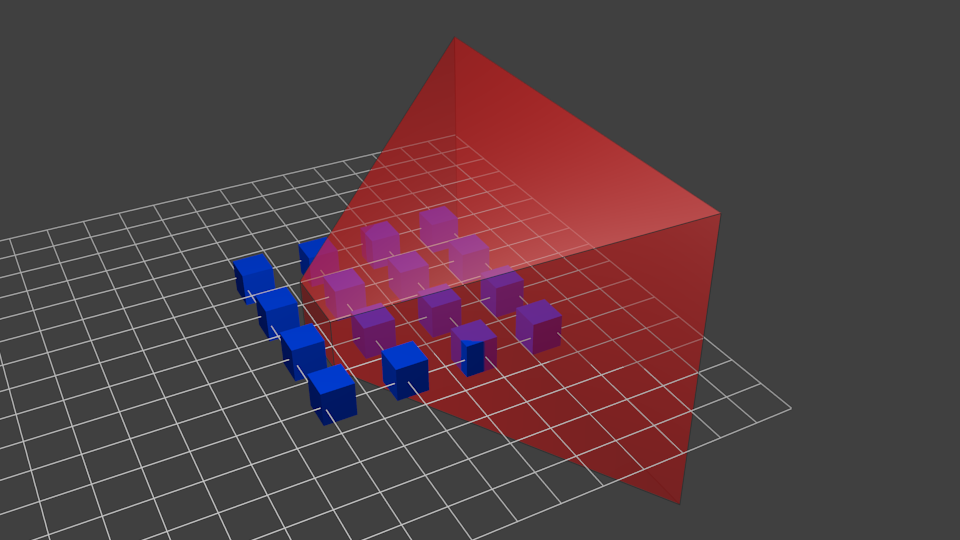
\includegraphics[width=0.8\textwidth]{images/nondeforme.png}
    \caption{Zentralprojektion}
    \label{fig:projection-sight-vol}
\end{figure}

\begin{figure}[H]
    \centering
    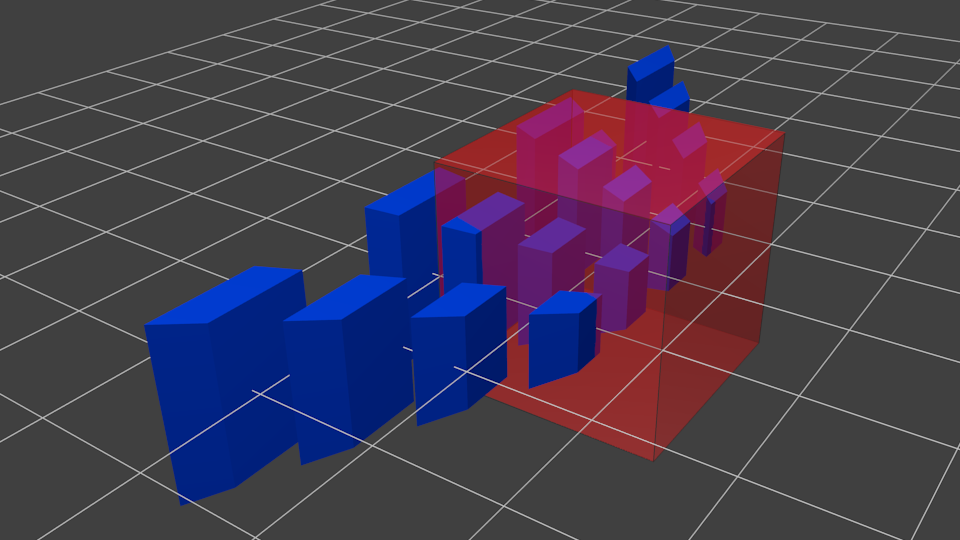
\includegraphics[width=0.8\textwidth]{images/deform.png}
    \caption{Zentralprojektion}
    \label{fig:projection-sight-vol}
\end{figure}

\subsubsection*{Windows-Viewport-Transformation}
Zuletzt müssen die zweidimensionalen Punkte noch mit Hilfe einer 
zweidimensionalen affinen Transformation in das Koordinatensystems des 
Anzeigenfensters auf dem Ausgabegerät transformiert werden. 
Diese Transformation wird auch Windows-Viewport-Transformation genannt.

\subsubsection{Rasterung}
\begin{figure}[H]
    \centering
    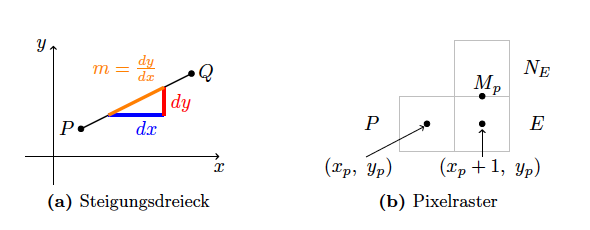
\includegraphics[width=1.0\textwidth]{images/bresenham.png}
    \caption{Rasterung nach Bresenham Algorithmus}
    \label{fig:screening-bresenham-line}
\end{figure}
Als Rasterung bezeichnet man das Transformieren kontinuierlicher, 
zweidimensionaler Daten auf diskrete Pixel.  
Anhand der gegebenen Daten muss also entschieden werden, welche Farbe ein Pixel des Ausgabegerätes erhält.
Wir haben also eine Funktion 
$Frame-Buffer: \mathbb{N} \times \mathbb{N} \to Farbe$. 
Die Pixel, die einem Dreieck zugeordnet werden, bezeichnet man auch als Fragment.

Im Bereich Echtzeitvisualisierung sind alle gängigen Rasterverfahren für 
Dreiecke und andere primitiven im wesentlichen Abwandlungen und 
Weiterentwicklungen von Algorithmen, die von Bresenham eingeführt wurden. 
Wir wollen uns den Bresenham Algorithmus für Linien/Strecken dazu exemplarisch 
anschauen.

\begin{Algorithmus}[Bresenham für Strecken mit positiver Steigung]
    \begin{figure}\centering
        \subfloat[Steigungsdreieck]{
            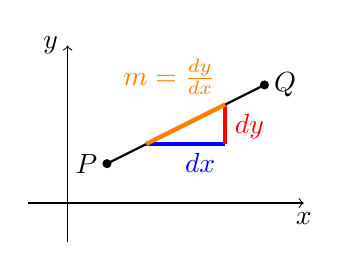
\begin{tikzpicture}[scale=1,]
                % axes
                \draw[->] (-.5, 0) -- (3, 0) coordinate (x axis);
                \node (x-label) at (x axis.south) [anchor=north] {$x$};
                \draw[->] (0, -.5) -- (0, 2) coordinate (y axis);
                \node (y-label) at (y axis.west) [anchor=east] {$y$};
                % S
                \draw[thick, black] (0.5, 0.5) coordinate (P) -- (2.5, 1.5) coordinate (Q);
                \filldraw [black] (P) circle (0.05cm);
                \node (P-label) at (P.west) [anchor=east] {$P$};
                \filldraw [black] (Q) circle (0.05cm);
                \node (Q-label) at (Q.east) [anchor=west] {$Q$};
                % triangle
                \draw[ultra thick, blue] (1, 3/4) -- ++(1, 0) coordinate (dx);
                \node (dx-label) at (dx.south west) [
                    anchor=north east, 
                    color=blue, 
                ] {$dx$};
                \draw[ultra thick, red] (dx) -- ++(0, 1/2) coordinate (dy);
                \node (dy-label) at (dy.south east) [
                    anchor=north west, 
                    color=red, 
                ] {$dy$};
                \draw[ultra thick, orange] (1, 3/4) -- ++(1, 1/2) coordinate (m);
                \node (m-label) at (m.west) [
                    anchor=south east, 
                    color=orange, 
                ] {$m = \frac{dy}{dx}$};
            \end{tikzpicture}
            \label{fig:screening-bresenham-triangle}
        }
        \hspace*{0.1\textwidth}
        \subfloat[Pixelraster]{
	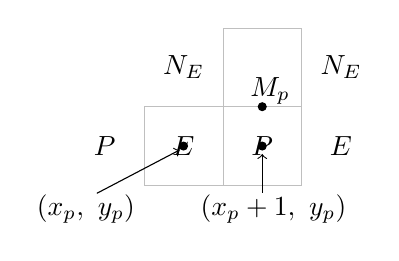
\begin{tikzpicture}
                \foreach \x / \y / \pxname in {-1/-1/P, 0/-1/E, 0/0/N_E} {
                    \draw [lightgray, very thin] (\x, \y) rectangle ++(1, 1);
                    \ifthenelse{\x < 0}{
                        \node (\pxname) at (\x-.5, \y+.5) {$\pxname$};
                    }{
                        \node (\pxname) at (\x+1.5, \y+.5) {$\pxname$};
                    }
                }
                \filldraw [black] (0.5, 0) circle (0.05cm);
                \node (M_p) at (0.6, 0.2) {$M_p$};
                \filldraw [black] (-0.5, -0.5) circle (0.05cm);
		\draw[<-] [black, thin] (-0.55, -0.55) --(-1.6, -1.1);
                \node (x0_y0) at (-1.4, -1) [
                    anchor=north east, 
                    outer sep=0pt, 
                    xshift=0.4cm, 
                ] {$\left( x_p,~ y_p \right)$};
                \filldraw [black] (0.5, -0.5) circle (0.05cm);
		\draw[<-] [black, thin] (0.5, -0.6) --(0.5, -1.1);
                \node (x1_y0) at (0, -1) [
                    anchor=north west, 
                    outer sep=0pt, 
                    xshift=-0.4cm, 
                ] {$\left( x_p + 1,~ y_p \right)$};
       	\end{tikzpicture}
        \label{fig:screening-bresenham-pixels}
        }
        \caption{Schrittbetrachtung Bresenham Algorithmus}
        \label{fig:screening-bresenham}
    \end{figure}
    Die Strecke $S = \overline{PQ} \in \mathbb{R}^n$ soll auf ein 
    ($n$-dimensionales Pixel-) Raster abgebildet werden (Siehe Abbildung 
    \ref{fig:screening-bresenham-line}). 
    Wir beschränken uns hier auf die Berechnung im $\mathbb{R}^2$. 
    $P$ und $Q$ seien gegeben mit 
    \begin{equation*}\begin{matrix}
        P = \begin{pmatrix} x_0 \\ y_0 \end{pmatrix} & 
        Q = \begin{pmatrix} x_1 \\ y_1 \end{pmatrix} & 
        \forall x_i, y_i \in \mathbb{R}
    \end{matrix}\end{equation*}
    Die Geradengleichung lässt sich einfach bestimmen (Abbildung 
    \ref{fig:screening-bresenham-triangle}):
    \begin{equation*}\begin{matrix}
        y & = & mx + b \\
        & \textrm{mit} & \\
        m & = & \frac{dy}{dx} \\
        dx & = & x_1 - x_0 \\
        dy & = & y_1 - y_0 \\
    \end{matrix}\end{equation*}
    Die Abbildung auf ein Raster ist für Steigungen 
    $m \in \left\{ 0,~ 1 \right\}$ trivial. 
    Anders für $0 < m < 1$. 
    Dafür betrachten wir in einem Schritt benachbarte Pixel 
    (Abbildung \vref{fig:screening-bresenham-pixels}): 
    \begin{itemize}
        \item Ausgangspixel $P\left( x_p,~ y_p \right)$
        \item Nachbar $E\left( x_p + 1,~ y_p \right)$
        \item ,,Nachfolgender'' Nachbar $N_E\left( x_p + 1,~ y_p + 1 \right)$
    \end{itemize}
    Der Mittelpunkt zwischen $N$ und $E$ wird festgelegt durch
    \begin{equation*}
        M_p = \left( x_p + 1,~ y_p + \frac{1}{2} \right)
    \end{equation*}
    Damit kann entschieden werden welches benachbarte Pixel zur Strecke gehört. 
    Liegt nun
    \begin{equation*}
        M_p ~\Big\{~ \begin{matrix}
            \textrm{oberhalb}~ \overline{PQ} &\Rightarrow& \textrm{wähle}~ E \\ 
            \textrm{unterhalb}~ \overline{PQ} &\Rightarrow& \textrm{wähle}~ N_E 
        \end{matrix}
    \end{equation*}\\
    Bresenham hat eine effiziente Lösung dieses Problems aufgezeigt.
    Zunächst lässt sich die Geradengleichung in eine Funktion $F$ umformen, die von 
    zwei Variablen abhängt: 
    \begin{equation*}\begin{matrix}
        y & = & \frac{dy}{dx} x + b \\
        dx \cdot y & = & dy \cdot x + dx \cdot b \\
        0 & = & dy \cdot x - dx \cdot y + dx \cdot b \\
        F\left(x,~ y\right) & := & dy \cdot x - dx \cdot y + dx \cdot b 
    \end{matrix}\end{equation*}
    Das arithmetische Entscheidungskriterium lautet also 
    \begin{equation*}\begin{matrix}
        (x,~ y) \in y = mx + b & \Leftrightarrow & F\left(x,~ y\right) = 0 \\
        & \textrm{bzw.} & \\
        F\left(x,~ y\right) & \Bigg\{ & \begin{matrix}
            = 0 & \left(x,~ y\right) \textrm{liegt auf}~ S \\
            > 0 & \left(x,~ y\right) \textrm{liegt unterhalb von}~ S \\
            < 0 & \left(x,~ y\right) \textrm{liegt oberhalb von}~ S \\
        \end{matrix}
    \end{matrix}\end{equation*}
    Damit kann die Entscheidungsfunktion $D_p$ definiert werden 
    \begin{equation*}\begin{matrix}
        D_p & := & 2 \cdot F\left(M_p\right) \\
        & = & 2 \cdot F\left(x_p + 1,~ y_p + \frac{1}{2}\right) \\
        & = & dy \left(2x_p + 2\right) - dx \left(2y_p + 1\right) + dx \cdot 2b
    \end{matrix}\end{equation*}
    1. Fall: $D_p < 0 ~\Rightarrow~$ Nachfolgepixel ist $E$
    \begin{equation*}\begin{matrix}
        D_E & = & 2 \cdot F\left(M_E\right) \\
        & = & 2 \cdot F\left(x_p + 2,~ y_p + \frac{1}{2}\right) \\
        & = & dy \cdot \left(2 x_p + 4\right) 
            - dx \cdot \left(2 y_p + 1\right) 
            + 2 \cdot b \cdot dx \\
        & = & D_p + \bigtriangleup_E \\
        & \textrm{mit} & \bigtriangleup_E := 2 \cdot dy
    \end{matrix}\end{equation*}
    2. Fall: $D_p \ge 0 ~\Rightarrow~$ Nachfolgepixel ist $NE$ \\
    \begin{equation*}\begin{matrix}
        D_{NE} & = & 2 \cdot F\left( M_{NE} \right) \\
        & = & D_p + \bigtriangleup_{NE} \\
        & \textrm{mit} & \bigtriangleup_{NE} := 2dy - 2dx
    \end{matrix}\end{equation*}
    Eine Implementierung könnte wie folgt aussehen: 
    \begin{lstlisting}[language=C]
bresenham(x0, y0, x1, y1){
    dx = x1 - x0;
    dy = y1 - y0;
    d = 2*dy - dx; /*F(x0 + 1,y0 + 1/2) | F(x0,y0)=0*/
    deltaE = 2 * dy;
    deltaNE = 2 * (dy - dx);
    x = x0;
    y = y0;
    writepixel(x0, y0);
    while (x < x1) {
        if (d < 0) {
            d += deltaE;
            x++;
        } else {
            d += deltaNE;
            x++; y++;
        }
        writepixel(x, y);
    }
}
    \end{lstlisting}
\end{Algorithmus}

Das Rastern erzeugt oft harte, kantige und ausgefranste Übergange. Diese Effekte bezeichnet man auch als Aliasing. Algorithmen, die diesen Aliasing-Effekten entgegenwirken nennt man auch Antialiasing. 
\begin{figure}[H]
    \centering
    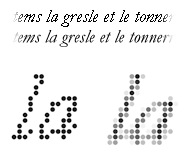
\includegraphics[width=0.5\textwidth]{images/Antialiasing.png}
    \caption{Eine Schrift mit und ohne Antialiasing}
    \label{fig:screening-antialiasing-font}
\end{figure}

\subsection*{Interpolation}
GLSL interpoliert Werte innerhalb eines Fragmentes linear zwischen den im Vertex-Shader gesetzten Werten.
Dies kann  zum Beispiel mit Hilfe eines Sweepline-Algorithmus realisiert werden.
\begin{figure}[H]
    \centering
    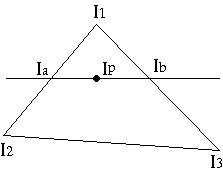
\includegraphics[width=0.5\textwidth]{images/gouraud_scanline.png}
    \caption{Scanline-Verfahren beim Gouraud-Shading}
    \label{fig:gouraud-shading-scanline}
\end{figure}


\subsection*{Sichtbarkeitsprobleme}

\subsubsection*{Clipping}
Beim 3D-Clipping werden alle Polygone verworfen, die nach der Transformation in Clipping-Koordinaten vollständig ausserhalb des Sichtvolumens
$[-1,1] \times [-1,1] \times [-1,1] $ liegen. Das 2D-Clipping findet nach der Projektion der Polygone statt. Polygone, die über das Viewportfenster hinaus ragen, werden an den Fensterkanten abgeschnitten.
Der wichtigste Schritt ist hierbei das Abschneiden von Strecken an diesen Kanten. Wir betrachten dazu exemplarisch den Cohen-Sutherland-Algorithmus:

\begin{Algorithmus}[Cohen-Sutherland]
\end{Algorithmus}

\subsubsection*{Culling/Rückseitenentfernung}
Als Culling bezeichnet man das Entfernen von Polygonen anhand Ihrer Orientierung, beziehungsweise Anhand der zugehörigen Normale. Man definiert, welche Orientierung eine Rückseite darstellt und verwirft dann Polygone, deren Normale positives beziehungsweise negatives Skalarprodukt mit der Blickrichtung aufweisen. So werden Beispielsweise Rückseiten, die nicht sichtbar sind, nicht weiter in der Pipeline verarbeitet.

\subsubsection* {z-Buffer}
Der Z-Buffer enthält für jedes Pixel $(u,v)$ nach der Rasterung  einen Wert zwischen $-1$ und $1$. Dieser Wert  ist der Abstand zum nächsten Punkt eines Polygons  in Clipping-Koordinaten von diesem Pixel auf der Projektionsebene.  Wir haben somit eine Funktion
\begin{align*}
Z-Buffer : \mathbb{N} \times \mathbb{N} \to [-1,1]  \; .
\end{align*}

\begin{figure}[H]
    \centering
    \includegraphics[width=1.0\textwidth]{images/gl_projectionmatrix_zbuffer_1.png}
    \caption{Z-Buffer-War}
    \label{fig:zbuffer-war}
\end{figure}



\begin{Algorithmus}[z-Buffer Algorithmus]
Setze Alle Einträge im Z-Buffer auf 1 (Hintergrund).
Setze alle Einträge im Framebuffer auf die Hintergrundfarbe. \\
$\forall$ Polygone P: \\
begin: \\
Transformiere das Polygon in Clipping-Koordinaten. \\
Transformiere das Polygon in Rasterkoordinaten. \\
$\forall$ erhaltenen Pixel (u,v): \\
begin: \\
$pz := $Z-Koordinate des Polygons in Clipping-Koordinaten zum entsprechenden Pixel \\
$zz:=$ Eintrag im Z-Buffer für das Pixel $(u,v)$ \\
if $pz < zz$: \\
begin: \\
$Z-Buffer(u,v) := pz$ \\
$Frame-Buffer(u,v) := Farbe(P,(u,v))$ \\
end \\
end \\
end
\end{Algorithmus}


\subsection{Lokale Beleuchtungsmodelle}
\subsubsection{Ideale und diffuse Reflexionen}
\subsubsection{Lambert  Modell}
Das Lambertsche Modell beschreibt, wie durch den perspektivischen Effekt die Strahlungsstärke mit flacher werdendem Abstrahlwinkel abnimmt. Sei nun $L$ der Punkt, an dem sich eine punktförmige Lichtquelle befindet und $P \in N$ ein Punkt eines Netzes $N$ mit Normale $n$ (also insbesondere gilt $||n|| = 1$).  Dann berechnet sich die Lichtintensität $I_d$ an diesem Punkt durch
\begin{align*}
I_d :=  I_l \cdot I_m \cdot max\biggl ( 0, \biggl< n, \frac{1}{||\overline{PL}||} \cdot \overline{PL} \biggr> \biggr)
\end{align*}
wobei $I_l \in [0,1]$ die Lichtintensität der Lichtquelle, $I_m \in [0,1]$ eine Materialkonstante und $max(a,b)$ das maximum der Zahlen $a$ und $b$ ist. 
Um die gesamte Lichtintensität zu berechnen wird noch ein konstanter, sogenannter ambienter Lichtanteil $I_a$ hinzuaddiert
\begin{align}
I := I_d + I_a \;.
\end{align} 
$I_a$ ist wie gesagt eine Konstante.
 Der Eindruck von ambienten Licht, also Licht, das aus keiner erkennbaren Richtung kommt und alles gleichmässig erhellt, entsteht durch Lichtstrahlen, die sehr oft an Gegenständen reflektiert werden.
Der Wert $I$ muss gegebenenfalls auf das Intervall $[0,1]$ beschränkt werden.
\begin{figure}[H]
    \centering
    \includegraphics[width=0.8\textwidth]{images/lambert.png}
    \caption{Lambert Modell diffuser Reflektion}
    \label{fig:reflection-lambert-diffuse-model}
\end{figure}

   
\subsubsection{Phong Modell}
Das Phong-Modell erweitert das  Lambert-Modell um den Effekt von spiegelnden Reflektionen. Die Idee ist, dass die Helligkeit zusätzlich zunimmt, je mehr die Betrachtungsrichtung dem perfekt reflektiertem Lichtstrahl entspricht.  

\begin{figure}[H]
    \centering
    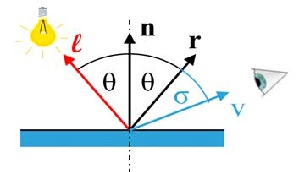
\includegraphics[width=0.6\textwidth]{images/phong_directions.jpg}
    \caption{Die einzelnen Komponenten des Phong-Modells}
    \label{fig:phong-directions}
\end{figure}

Ist $v$ der normierte Vektor in Richtung Kamera und $l$ der normierte Vektor in Richtung Lichtquelle, dann definiert man die  reflektierende Lichtintensität durch
\begin{align}
I_s := I_l \cdot I_m \cdot s \cdot \max\biggl ( 0, <r,v>^h \biggr)\;.
\end{align}
$I_l$ ist hierbei wieder die Intensität der Lichtquelle und $I_m$ eine Materialkonstante. Beide liegen in einen Wertebereich von $[0,1]$ 
$h$ ist eine ganze Zahl im Wertebereich $[0, \infty)$ und bestimmt die "härte" der Reflexion. $s$ ist eine Fließkommazahl im Wertebereich $(0,1]$ und beeinflusst den Glanz der Oberfläche.
 Der Vektor $r$ lässt sich berechnen durch 
\begin{align}
r = -l + 2 \cdot <n, l> \cdot n
\end{align}
wobei $n$ die Normale an dem betrachteten Oberflächenpunkt ist.

\begin{figure}[H]
    \centering
    \includegraphics[width=0.8\textwidth]{images/phong.png}
    \caption{Phong Modell spiegelnder Reflektion}
    \label{fig:reflection-phong-specular-model}
\end{figure}

Im Phong-Modell wird nun die endgültige Lichtentität wie folgt zusammengesetzt:

\begin{align}
I := I_s + I_d + I_a
\end{align}
wobei $I_d$ die diffuse Lichtintensität aus dem Lambert-Modell und $I_a$ den konstanten, ambienten Anteil bedeutet.
Gegebenenfalls muss $I$ wieder auf das Intervall $[0,1]$ beschränkt werden.

\begin{figure}[H]
    \centering
    \includegraphics[width=1.0\textwidth]{images/Phong_Components.png}
    \caption{Die einzelnen Komponenten des Phong-Modells}
    \label{fig:phong-components}\end{figure}

Die Möglichkeiten, ein bestimmtes Material zu beschreiben, sind  beim Phong-Modell beschränkt. 
Es gibt komplexere lokale Beleuchtungsmodelle, wie zum Beispiel das Cook-Torrente-Modell, die eine detaillierte Materialbeschreibung zulassen.




\subsection{Shader und standard Algorithmen}
\subsubsection{Mittelung der Normalen}
Stoßen mehrere Flächen mit Normalen $\{ N_1, N_2, \cdots, N_k \}$ an einem Vertex $V$ zusammen, so  bezeichnen wir  mit
$\bar{N}_V:= \frac{1}{k}\sum N_i$ die gemittelte Normale.
\begin{figure}[H]
    \centering
    \includegraphics[width=0.5\textwidth]{images/gouraud_normals.png}
    \caption{Verschiedene Normalen von angrenzenden Flächen}
    \label{fig:gouraud-shading-scanline}
\end{figure}

\subsubsection{Flat-Shading, Gouraud und Phong Shading}
\begin{figure}[H]
    \centering
    \includegraphics[width=1.0\textwidth]{images/flat_gouraud_phong.jpg}
    \caption{Flat, Gouraud und Phong-Shading}
    \label{fig:shading-flat-phong-models}
\end{figure}
  \begin{lstlisting}
  \end{lstlisting}

Man spricht vom Flat-Shading, wenn keine Interpolation der Helligkeitswerte innerhalb eines Dreiecks durchgeführt wird, sondern der gleiche Wert für das gesamte Dreieck verwendet wird.
Es gibt zwei prominente Möglichkeiten, die Helligkeitswerte zu interpolieren, das  Gouraud und das Phong Shading. 

\subsubsection{Texturen und UV-Mapping}
\begin{figure}[H]
    \centering
    \includegraphics[width=1.0\textwidth]{images/tm_uv.png}
    \caption{uv mapping} %TODO: fix caption&label
    \label{fig:uv-mapping1}
\end{figure}

\begin{figure}[H]
    \centering
    \includegraphics[width=1.0\textwidth]{images/tm_face.jpg}
    \caption{uv mapping} %TODO: fix caption&label
    \label{fig:uv-mapping2}
\end{figure}




\subsubsection{Bumpmapping}
Die relativen Höheninformationen liegen in einer Textur in Form von Graustufen vor – der sogenannten Heightmap. Jeder Grauwert steht für eine bestimmte Höhe. Normalerweise ist Schwarz (Wert 0) die „tiefste“ Stelle und Weiß (Wert: 255) die „höchste“.  Bei der Lichtberechnung, die wesentlich von der Normale abhängt, wird die gegebene Normale so abgeändert, als gäbe es eine Vertiefung bzw. eine Erhöhung entsprechend der Höheninformation.  Da Höhenunterschiede nur durch Veränderung der Helligkeit vorgegaukelt werden, die Flächen aber glatt bleiben, treten einige sichtbare Fehler auf:
Bei flachem Betrachtungswinkel wirkt die Struktur stark verzerrt.
Die Silhouette bleibt so eben wie beim ursprünglichen Objekt.
Es wird ein glatter Schatten geworfen.
Bumps werfen keine Schatten aufeinander.

\begin{figure}[H]
    \centering
    \includegraphics[width=1.0\textwidth]{images/Bumpmap.png}
    \caption{uv mapping} %TODO: fix caption&label
    \label{fig:uv-mapping3}
\end{figure}




\subsubsection{Displacementmapping}
Wie beim Bumpmapping  wird  eine Height-map als Textur mitgegeben.
Im Gegensatz dazu werden die Punkte des Gitternetzes (Vertices)  entsprechend diesen Texturinformationen entlang ihrer Normalen, das heißt senkrecht zur Oberfläche, tatsächlich verschoben. So ist es beispielsweise möglich, ein Höhenrelief durch das Anwenden einer Displacement Map auf eine ebene (planare) Oberfläche zu übertragen und dieser damit eine raue Struktur zu verleihen. Zusätzlich zur Verschiebung kann in Abhängigkeit von der Dichte des Drahtgitters dessen Verfeinerung notwendig werden. Man spricht dann von Tesselation.

\begin{figure}[H]
    \centering
    \includegraphics[width=0.5\textwidth]{images/Displacement.jpg}
    \caption{Displacementmapping} %TODO: fix caption&label
    \label{fig:displacement-mapping}
\end{figure}



\subsubsection{Shadowmap}
Das Rendern einer Szene mit Schatten unter Zuhilfenahme von einer Shadow Map geschieht im Wesentlichen in zwei Schritten. Als erstes wird die Szene aus der Sicht des Lichts gerendert und die Tiefeninformation (z-Buffer) in eine Textur gerendert. Anschließend wird die Szene normal gerendert, wobei für jedes Pixel  der Abstand des zugehörigen Vertex zur Lichtquelle (in Clipping Coordinaten) mit dem Wert der Shadow Map verglichen wird. Ist der Wert in der Shadow Map kleiner, wird  das Pixel schattiert gerendert.

\begin{figure}[H]\centering
    \subfloat[Tiefeninformation aus Sicht des Lichtes gerendert]{
        \hspace*{0.05\textwidth}
         \includegraphics[width=0.5\textwidth]{images/sm_zb.png}
    \label{fig:shadowmap3}
    }
    \hspace*{0.1\textwidth}
    \subfloat[Rendering ohne Shadow mapt]{
        \includegraphics[width=0.5\textwidth]{images/sm_ns.png}
    \label{fig:shadowmap1}
    }
    \vspace*{1em}
    \subfloat[Rendering mit Shadow map]{
        \hspace*{0.05\textwidth}
         \includegraphics[width=0.5\textwidth]{images/sm_ws.png}
    \label{fig:shadowmap2}
    }
\end{figure}



Probleme bereitet der sogenannte z-Buffer War. Abhilfe schafft eine transformation der z-Buffer-Werte durch eine geeignete Funktion.



\subsubsection{ Forward shading, Blending und Transparenz}
Beim Forward shading wird die Lichtberechnung für jedes Vertex in dem entsprechen shader durchgeführt. Im Gegensatz dazu vergleiche deferred shading.
Werden mehrere Render passes durchgeführt, so kann man über das Blending festlegen, wie die doppelten Fragmente gemischt werden.
Transparenz kann man zum Beispiel realisieren, indem man die transparenten Objekte mit entsprechendem Blending über die vorher gerenderten  Szene rendert.
Ein lineares Blending wird zum Beispiel durch die Funktion 
\begin{align}
p_{neu} = \alpha \cdot p_1 + (1- \alpha)p_2
\end{align}
realisiert. Mehrere Lichtquellen können entweder direkt im Shader oder durch mehrfaches Rendern der Szene mit den verschiedenen Lichtquellen und entsprechendem Blending realisiert werden.
\subsubsection{Deferred shading}
Der Begriff Deferred Shading (zu dt. "verzögertes Schattieren") oder auch Deferred Lighting ("verzögerte Beleuchtung") beschreibt eine Technik, mit deren Hilfe die Geometrieverarbeitung von der Lichtberechnung getrennt werden kann. Dies erlaubt hunderte Lichtquellen in einer hoch-komplexen Szene.


Um eine Szene mit einem traditionellen Forward-Renderer zu beleuchten, wird normalerweise jedes Objekt der Szene mit den entsprechenden Beleuchtungsparametern der Lichtquelle gezeichnet. 
Die Lichtberechnungen werden für jedes Vertex aufgerufen.

Deferred Shading verfolgt einen anderen Ansatz: Für jeden Pixel werden die Daten aus dem G-Buffer ausgelesen und die Beleuchtung entsprechend dieser Daten im Fragmentshader einer minimalen, bildschirmfüllenden Geometrie berechnet. 


\begin{figure}[H]
    \centering
    \includegraphics[width=1.0\textwidth]{images/deffered_shading.jpg}
    \caption{G-Buffer beim deferred shading} %TODO: fix caption&label
    \label{fig:defferedshading}
\end{figure} 

Mit dieser Methode sind hunderte Lichter gleichzeitig in einer hoch-komplexen Szene möglich.
Der Vorteil ist, dass die Lichtberechnungen somit nur für wirklich sichtbaren Pixel des tatsächlichen Ausgebe-Bildes  berechnet werden.
Das Verfahren ist nur dann sinnvoll, wenn man es mit einer sehr komplexen Geometrie und sehr vielen Lichtquellen zu tun hat. 

\begin{figure}[H]
    \centering
    \includegraphics[width=0.8\textwidth]{images/deferred_v2.png}
    \caption{Pipeline beim deferred rendering} %TODO: fix caption&label
    \label{fig:defferedshading}
\end{figure}



\begin{figure}[H]
    \centering
    \includegraphics[width=0.8\textwidth]{images/deferred_shading_off.jpg}
    \caption{Szene gerendert mit forward shading. } %TODO: fix caption&label
    \label{fig:defferedshading}
\end{figure}



\begin{figure}[H]
    \centering
    \includegraphics[width=0.8\textwidth]{images/deferred_shading_on.jpg}
    \caption{Szene gerendert mit  deferred shading. Der verbesserte  Eindruck des Tageslichtes wird durch eine sehr hohe Anzahl von Lichtquellen erzeugt.} %TODO: fix caption&label
    \label{fig:defferedshading}
\end{figure}



\subsection{GLSL via WebGL}
\subsubsection{Minimaler Shader}
Minimaler Shader auf bildschirmfüllender Minimal-Geometrie
   \begin{lstlisting}
<!DOCTYPE html>
<!--
To change this license header, choose License Headers in Project Properties.
To change this template file, choose Tools | Templates
and open the template in the editor.
-->
<html>
    <head>
        <title>TODO supply a title</title>
        <meta charset="UTF-8">
        <meta name="viewport" content="width=device-width, initial-scale=1.0">
    </head>
    <body>
        <canvas id="glcanvas"></canvas>

        <script id="2d-vertex-shader" type="x-shader/x-vertex">
            attribute vec2 a_position;
            uniform float t;
            varying float T;
            void main() {
            //  gl_Position = vec4(a_position, 0.0, t);
            T = t;
            gl_Position = vec4(a_position[0], a_position[1], 0.0, 1.0);
            }
        </script>

        <script id="2d-fragment-shader" type="x-shader/x-fragment">
            precision mediump float;
            varying float T;
            void main() {
            gl_FragColor = vec4(0.0 ,1.0,0.0,1.0);

            }
        </script>


        <script type="text/javascript">


            var shaderScript;
            var shaderSource;
            var vertexShader;
            var fragmentShader;
            var program;
            var canvas;
            var gl;
            var buffer;
            window.onload = init;


            var someProgress;

            function init() {
            // Get A WebGL context
            canvas = document.getElementById("glcanvas");
            canvas.width = 400;
            canvas.height = 300;



            gl = canvas.getContext("webgl");


            gl.viewport(0, 0, gl.drawingBufferWidth, gl.drawingBufferHeight);


            //compile and link shaders
            shaderScript = document.getElementById("2d-vertex-shader");
            shaderSource = shaderScript.text;


            vertexShader = gl.createShader(gl.VERTEX_SHADER);
            gl.shaderSource(vertexShader, shaderSource);
            gl.compileShader(vertexShader);

            shaderScript = document.getElementById("2d-fragment-shader");
            shaderSource = shaderScript.text;
            fragmentShader = gl.createShader(gl.FRAGMENT_SHADER);
            gl.shaderSource(fragmentShader, shaderSource);
            gl.compileShader(fragmentShader);

            program = gl.createProgram();
            gl.attachShader(program, vertexShader);
            gl.attachShader(program, fragmentShader);
            gl.linkProgram(program);






            // Create an empty buffer
            buffer = gl.createBuffer();

            someProgress = 1.0;

            //start gameloop
            render();
            }

            function render() {

            //recusrive gameloop/animation frame offered by browser
            window.requestAnimationFrame(render);


            //clear background and paint it red
            gl.clearColor(1.0, 0.0, 0.0, 1.0);

            gl.clear(gl.COLOR_BUFFER_BIT);



            //use shader program
            gl.useProgram(program);



            //bind geometry to sahder program
            gl.bindBuffer(gl.ARRAY_BUFFER, buffer);

            gl.bufferData(
            gl.ARRAY_BUFFER,

            //data array values
            new Float32Array([
            -1.0, -1.0,
            1.0, -1.0,
            -1.0, 1.0,
            -1.0, 1.0,
            1.0, -1.0,
            1.0, 1.0]),

            gl.STATIC_DRAW);

            positionLocation = gl.getAttribLocation(program, "a_position");
            gl.enableVertexAttribArray(positionLocation);

            gl.vertexAttribPointer(positionLocation, 2, gl.FLOAT, false, 0, 0);



            var tLocation = gl.getUniformLocation(program, "t");
            gl.uniform1f(tLocation, someProgress);

            someProgress += 0.01;

            gl.drawArrays(gl.TRIANGLES, 0, 6);
            }
        </script>




    </body>
</html>
    \end{lstlisting}
